{
  \newmdenv[tikzsetting={draw=black,fill=white,fill opacity=0.7, line width=4pt},backgroundcolor=none,leftmargin=0,rightmargin=0,innertopmargin=4pt,skipbelow=\baselineskip,%
  skipabove=\baselineskip]{TitleBoxAbstraction}

  \usebackgroundtemplate{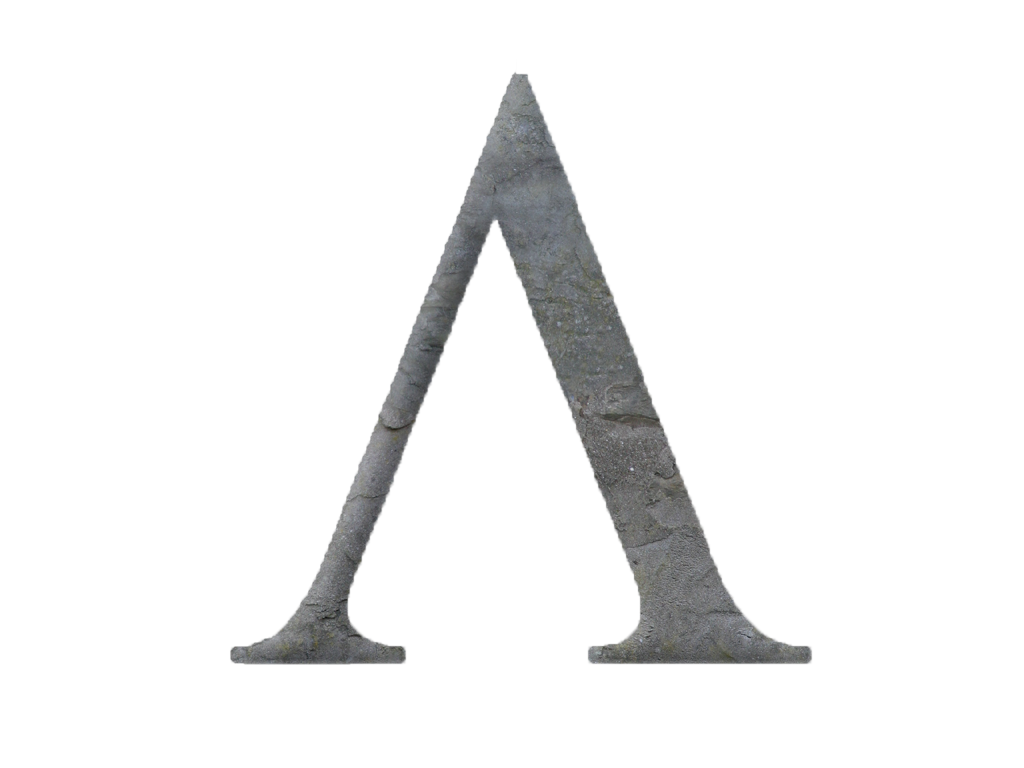
\includegraphics[width=1.0\paperwidth]{image/title-background.png}}

  \begin{frame}[plain] 
  \title{Abstraction}
  
  \vspace{3em}

  \begin{TitleBoxAbstraction}
    \begin{center}
    {\Large \inserttitle}
    \end{center}
  \end{TitleBoxAbstraction}

  \end{frame}
}



\begin{frame}
\frametitle{Principles and Goals of Abstraction}
\begin{block}{Construct a constraint}
\begin{itemize}
  \item minimise the requirements to satisfy the constraint to increase instances
  \item maximise potential for deriving operations as a consequence of satisfying the constraint 
\end{itemize}
\end{block}
\end{frame}


\begin{frame}
\frametitle{Principles and Goals of Abstraction}
\begin{block}{Trade-off between the two}
\begin{itemize}
  \item stronger constraint
    \begin{itemize}
      \item fewer instances
      \item more derived operations
    \end{itemize}
  \item weaker constraint
    \begin{itemize}
      \item more instances
      \item fewer derived operations
    \end{itemize}
\end{itemize}
\end{block}
\end{frame}


\begin{frame}
\frametitle{Principles and Goals of Abstraction}
\begin{block}{The ultimate goal}
Avoid repetition of the same work
\end{block}
\end{frame}


\begin{frame}
\frametitle{Principles and Goals of Abstraction}
\begin{block}{Consequently}
A proposed abstraction that loses in both directions is a \emph{false economy} and must be efficiently discarded.
\end{block}
\tiny{\emph{cough} \lstinline{scala.collection.generic.CanBuildFrom} \emph{cough}}\normalsize
\end{frame}


\begin{frame}
\frametitle{Abstraction}
\begin{center}
\huge{For example}\normalsize
\end{center}
\end{frame}

%%%

{
  \newmdenv[tikzsetting={draw=black,fill=white,fill opacity=0.7, line width=4pt},backgroundcolor=none,leftmargin=0,rightmargin=0,innertopmargin=4pt,skipbelow=\baselineskip,%
  skipabove=\baselineskip]{TitleBoxWhatDoesMonadMean}

  \usebackgroundtemplate{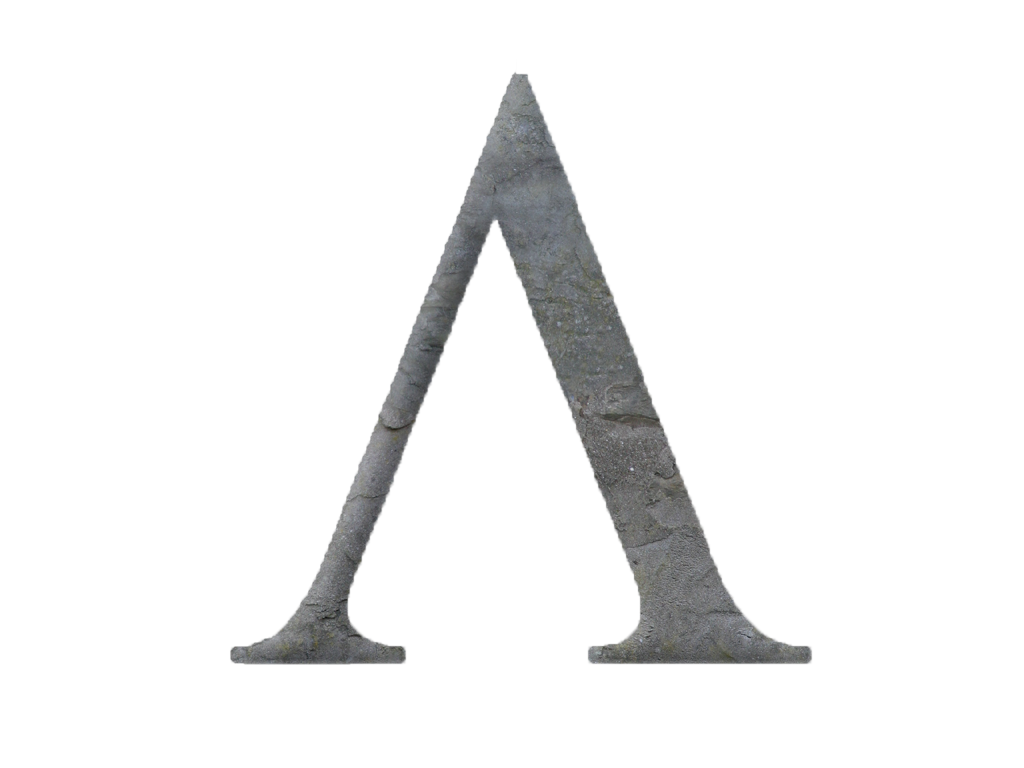
\includegraphics[width=1.0\paperwidth]{image/title-background.png}}

  \begin{frame}[plain] 
  \title{What Does Monad Mean?}
  
  \vspace{3em}

  \begin{TitleBoxWhatDoesMonadMean}
    \begin{center}
    {\Large \inserttitle}
    \end{center}
  \end{TitleBoxWhatDoesMonadMean}

  \end{frame}
}


\begin{frame}
\frametitle{What Does Monad Mean?}
\begin{block}{Well if you google it}
burritos, spacesuits or some silly shenanigans like that
\end{block}
% wrong question
\end{frame}


\begin{frame}[fragile]
\frametitle{Monad}
\begin{block}{But if we decline the distraction}
\begin{lstlisting}[style=scala,mathescape]
trait Monad[F[_]] {
  def bind[A, B]
    (f: A => F[B]):
    F[A] => F[B]
  def unit[A]:
    A => F[A]
}
\end{lstlisting}
\end{block}
\end{frame}


\begin{frame}[fragile]
\frametitle{Monad}
\begin{block}{This abstraction has many instances (values for \lstinline$F$)}
\begin{itemize}
  \item list
  \item continuations
  \item nullable values
  \item exception chaining
  \item state
  \item I/O actions
  \item argument threading
  \item logging
  \item \emph{hundreds more}
\end{itemize}
\end{block}
\end{frame}


\begin{frame}
\frametitle{Monad}
\begin{block}{This abstraction gives us many useful operations}
\begin{itemize}
  \item sequencing a list of effect values

        \lstinline$List[F[A]] -> F[List[A]]$
  \item replicating an effect a given number of times

        \lstinline$Int -> F[A] -> F[List[A]]$
  \item \emph{bazillions more}
\end{itemize}
\end{block}
\end{frame}


\begin{frame}
\frametitle{Monad}
\begin{block}{We just saw}
\begin{itemize}
  \item<1> the monad abstraction expressed as a constraint
  \item<2> instances that satisfy the constraint
  \item<3> operations that are derived from the constraint
\end{itemize}
\end{block}
\end{frame}


\begin{frame}
\frametitle{Abstraction nomenclature}
\begin{block}{Other abstractions trade off along the two competing principles}
\begin{itemize}
  \item covariant functor
  \item applicative functor
  \item semigroupoid
  \item comonad
  \item profunctor
  \item monoid
  \item \emph{hundreds more}
\end{itemize}
\end{block}
\end{frame}


\begin{frame}
\frametitle{Now that we know this}
\begin{block}{We can do some mythbusting}
\begin{itemize}
  \item<1-> Monads are for side-effects
  \item<2-> Monads are for functional programming only
  \item<3-> Monads are for doing I/O
  \item<4-> Monads don't apply to my programming tasks
  \item<5-> Monads are for those who want Scala to be like Haskell
\end{itemize}
\visible<6->{
  \begin{tikzpicture}[remember picture,overlay]
  \coordinate (aa) at ($(a1)+(1,4.5)$);
  \node[right] at (aa) {
\includegraphics[height=3cm]{image/bullshizzles.png}};
  \end{tikzpicture}
}
\end{block}
\end{frame}
